\documentclass[border=4pt]{standalone}
\usepackage{tikz}
\usepackage{pgfplots}
\pgfplotsset{compat=1.17}
\usepackage[table]{xcolor}
\usetikzlibrary{shapes.geometric, arrows.meta, positioning, fit, calc}
\definecolor{headingblue}{HTML}{1F4E79}
\definecolor{lightblue}{HTML}{D9EAF7}
\definecolor{softgray}{HTML}{F4F6F8}
\definecolor{darkgray}{HTML}{404040}
\definecolor{prismagreen}{HTML}{E8F5E9}
\definecolor{prismabox}{HTML}{1565C0}
\definecolor{chartblue}{HTML}{2196F3}
\definecolor{chartorange}{HTML}{FF9800}
\definecolor{chartgreen}{HTML}{4CAF50}
\definecolor{chartred}{HTML}{F44336}
\definecolor{chartpurple}{HTML}{9C27B0}
\definecolor{chartgray}{HTML}{9E9E9E}
\begin{document}
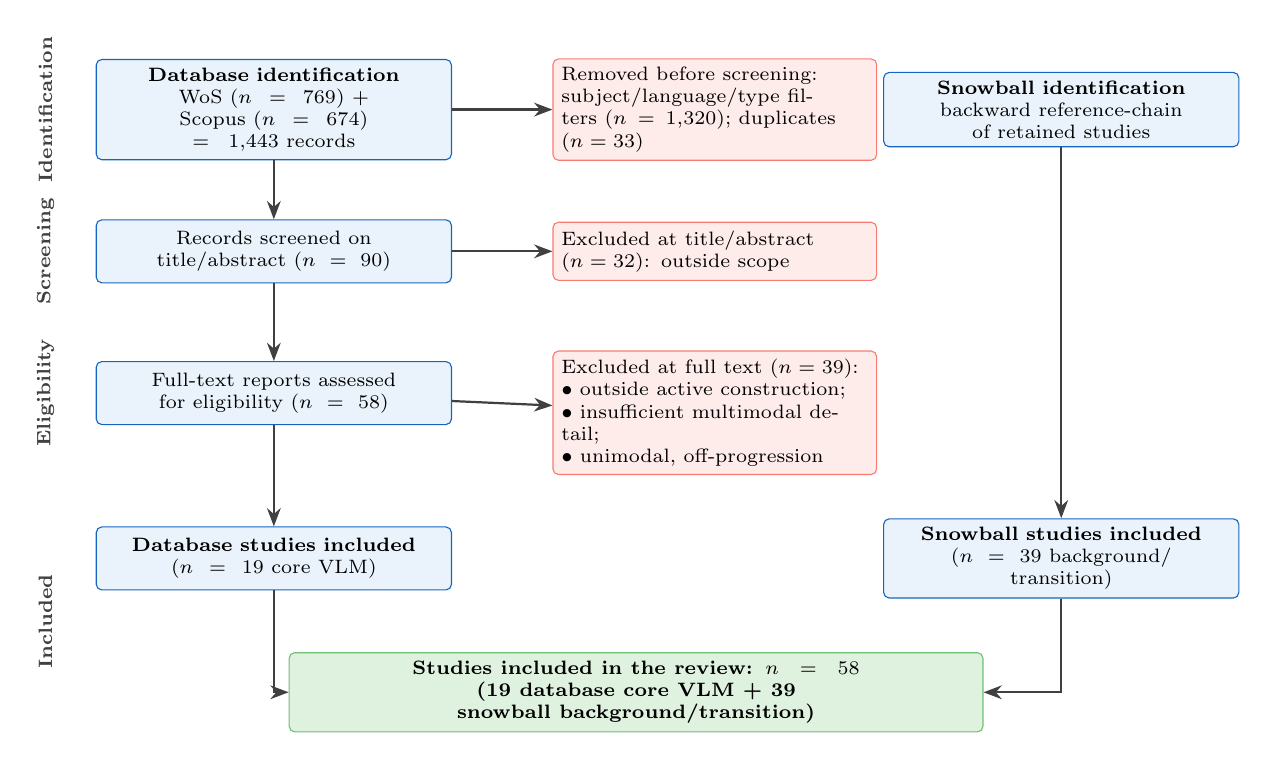
\begin{tikzpicture}[
  box/.style={rectangle, draw=prismabox, fill=lightblue!55, text width=4.3cm, align=center, minimum height=0.8cm, font=\scriptsize, rounded corners=2pt, inner sep=3pt},
  excl/.style={rectangle, draw=chartred!70, fill=chartred!10, text width=3.9cm, align=left, minimum height=0.7cm, font=\scriptsize, rounded corners=2pt, inner sep=3pt},
  final/.style={rectangle, draw=chartgreen!80, fill=chartgreen!18, text width=8.6cm, align=center, minimum height=0.9cm, font=\scriptsize\bfseries, rounded corners=2pt, inner sep=3pt},
  stage/.style={font=\scriptsize\bfseries\color{darkgray}, align=center, rotate=90},
  arr/.style={-Stealth, thick, color=darkgray},
]
% --- Database track (left) ---
\node[box] (dbid) at (0,0) {\textbf{Database identification}\\ WoS ($n=769$) + Scopus ($n=674$)\\ $=1{,}443$ records};
\node[excl] (dbpre) at (5.6,0) {Removed before screening: subject/language/type filters ($n=1{,}320$); duplicates ($n=33$)};
\node[box] (dbscr) at (0,-1.8) {Records screened on\\ title/abstract ($n=90$)};
\node[excl] (dbscrx) at (5.6,-1.8) {Excluded at title/abstract\\ ($n=32$): outside scope};
\node[box] (dbft) at (0,-3.6) {Full-text reports assessed\\ for eligibility ($n=58$)};
\node[excl] (dbftx) at (5.6,-3.85) {Excluded at full text ($n=39$):\\ $\bullet$ outside active construction;\\ $\bullet$ insufficient multimodal detail;\\ $\bullet$ unimodal, off-progression};
\node[box] (dbinc) at (0,-5.7) {\textbf{Database studies included}\\ ($n=19$ core VLM)};

% --- Snowball track (right) ---
\node[box] (sbid) at (10.0,0) {\textbf{Snowball identification}\\ backward reference-chain\\ of retained studies};
\node[box] (sbinc) at (10.0,-5.7) {\textbf{Snowball studies included}\\ ($n=39$ background/\\ transition)};

% --- Merge ---
\node[final] (final) at (4.6,-7.4) {Studies included in the review: $n=58$\\ (19 database core VLM + 39 snowball background/transition)};

% --- arrows ---
\draw[arr] (dbid) -- (dbpre);
\draw[arr] (dbid) -- (dbscr);
\draw[arr] (dbscr) -- (dbscrx);
\draw[arr] (dbscr) -- (dbft);
\draw[arr] (dbft) -- (dbftx);
\draw[arr] (dbft) -- (dbinc);
\draw[arr] (sbid) -- (sbinc);
\draw[arr] (dbinc.south) |- (final.west);
\draw[arr] (sbinc.south) |- (final.east);

% --- stage labels ---
\node[stage] at (-2.9,0) {Identification};
\node[stage] at (-2.9,-1.8) {Screening};
\node[stage] at (-2.9,-3.6) {Eligibility};
\node[stage] at (-2.9,-6.5) {Included};
\end{tikzpicture}
\end{document}
